
                \begin{figure}
                    \centering
                    \begin{tikzpicture}
                        \pgfplotsset{%
                            width=1\textwidth,
                            height=0.4\textheight
                        }
                        \begin{axis}[
                            xlabel={Runs since restart},
                            ylabel={Average dynamic energy (watt)},
                            ymin=0,ymax=70,
                        ]
                        
                            \addplot [mark=none, densely dashed, red]  coordinates {
                            (1, 41.67564618327381)(2, 39.68165239562263)(3, 48.48481613397879)(4, 40.78598578951857)(5, 40.50253578458274)
                            };
                            \addlegendentry{workstation - IntelPowerGadget}
                            
                            \addplot [mark=none, densely dashed, blue]  coordinates {
                            (1, 41.772671471799335)(2, 40.38545683070729)(3, 40.30687766861954)(4, 40.63625225322694)(5, 40.25174331481879)
                            };
                            \addlegendentry{workstation - HardwareMonitor}
                            
                            \addplot [mark=none, densely dashed, cyan]  coordinates {
                            (1, 36.02602024964694)(2, 33.933571207200366)(3, 31.013160496170958)(4, 35.7314842561267)(5, 31.18544315034984)
                            };
                            \addlegendentry{workstation - Clamp (win)}
                            
                        \end{axis}
                    \end{tikzpicture} 
                \caption{A graph illustrating the energy consumption of Cores for test case FannkuchRedux with regards to how long ago the DUT was restarted, experiment \#2, (with outliers)} \label{fig:FannkuchRedux_Cores_iteration_exp2}
                \end{figure}
                